\documentclass[a4 paper]{article}
\usepackage[inner=2.0cm,outer=2.0cm,top=2.5cm,bottom=2.5cm]{geometry}
\usepackage{setspace}
\usepackage[rgb]{xcolor}
\usepackage{verbatim}
\usepackage{subcaption}
\usepackage{amsgen,amsmath,amstext,amsbsy,amsopn,tikz,amssymb}
\usepackage{fancyhdr}
\usepackage[colorlinks=true, urlcolor=blue,  linkcolor=blue, citecolor=blue]{hyperref}
\usepackage[colorinlistoftodos]{todonotes}
\usepackage{rotating}
\usepackage{booktabs}
\newcommand{\ra}[1]{\renewcommand{\arraystretch}{#1}}

\newtheorem{thm}{Theorem}[section]
\newtheorem{prop}[thm]{Proposition}
\newtheorem{lem}[thm]{Lemma}
\newtheorem{cor}[thm]{Corollary}
\newtheorem{defn}[thm]{Definition}
\newtheorem{rem}[thm]{Remark}
\numberwithin{equation}{section}

\newcommand{\homework}[6]{
   \pagestyle{myheadings}
   \thispagestyle{plain}
   \newpage
   \setcounter{page}{1}
   \noindent
   \begin{center}
   \framebox{
      \vbox{\vspace{2mm}
    \hbox to 6.28in { {\bf CSE 211:~Discrete Mathematics \hfill {\small (#2)}} }
       \vspace{6mm}
       \hbox to 6.28in { {\Large \hfill #1  \hfill} }
       \vspace{6mm}
       \hbox to 6.28in { {\it Instructor: {\rm #3} \hfill  {\rm #5} \hfill  {\rm #6}} \hfill}
       \hbox to 6.28in { {\it Assistant: #4  \hfill #6}}
      \vspace{2mm}}
   }
   \end{center}
   \markboth{#5 -- #1}{#5 -- #1}
   \vspace*{4mm}
}

\newcommand{\problem}[2]{~\\\fbox{\textbf{Problem #1}}\hfill (#2 points)\newline\newline}
\newcommand{\subproblem}[1]{~\newline\textbf{(#1)}}
\newcommand{\D}{\mathcal{D}}
\newcommand{\Hy}{\mathcal{H}}
\newcommand{\VS}{\textrm{VS}}
\newcommand{\solution}{~\newline\textbf{\textit{(Solution)}} }

\newcommand{\bbF}{\mathbb{F}}
\newcommand{\bbX}{\mathbb{X}}
\newcommand{\bI}{\mathbf{I}}
\newcommand{\bX}{\mathbf{X}}
\newcommand{\bY}{\mathbf{Y}}
\newcommand{\bepsilon}{\boldsymbol{\epsilon}}
\newcommand{\balpha}{\boldsymbol{\alpha}}
\newcommand{\bbeta}{\boldsymbol{\beta}}
\newcommand{\0}{\mathbf{0}}


\begin{document}
\homework{Homework \#1}{Due: 17/11/20}{Dr. Zafeirakis Zafeirakopoulos}{Gizem S\"ung\"u}{}{}
\textbf{Course Policy}: Read all the instructions below carefully before you start working on the assignment, and before you make a submission.
\begin{itemize}
\item It is not a group homework. Do not share your answers to anyone in any circumstance. Any cheating means at least -100 for both sides. 
\item Do not take any information from Internet.
\item No late homework will be accepted. 
\item For any questions about the homework, send an email to gizemsungu@gtu.edu.tr
\item The homeworks (both latex and pdf files in a zip file) will be
submitted into the course page of Moodle.
\item The latex, pdf and zip files of the homeworks should be saved as
"Name\_Surname\_StudentId".$\{$tex, pdf, zip$\}$.
\item If the answers of the homeworks have only calculations without any formula or any explanation -when needed- will get zero.
\item Writing the homeworks on Latex is strongly suggested. However, hand-written paper is still accepted $\textbf{IFF}$ hand writing of the student is clear and understandable to read, and the paper is well-organized. Otherwise, the assistant cannot grade the student's homework.
\end{itemize}

\problem{1: Conditional Statements}{5+5+5=15}
State the converse, contrapositive, and inverse of each of these conditional statements.


\subproblem{a} If it snows tonight, then I will stay at home.
\solution
%%%%%%REMOVE \newline commands while writing your answer%%%%%
\newline
p=if it snows tonight, q=i will stay at home.
\newline
The statement is $p\Rightarrow q$
\newline
\textbf{Converse:}
\newline
The converse of statement p $\Rightarrow q$ is $q\Rightarrow p.$
Converse is that "If i will stay at home, then it snows tonight".
\newline
\textbf{Contrapositive:}
\newline
The contrapositive of statement p $\Rightarrow q$ is $q' \Rightarrow p'.$
\newline
contrapositive is that" If i will not stay at home, then it does not snow tonight".
\newline
\textbf{Inverse:}
\newline
The inverse of statement p $\Rightarrow q$ is $p'\Rightarrow q'.$
\newline
inverse is that "if it doesnt snow tonight, then i will not stay at home."
\newline



\subproblem{b} I go to the beach whenever it is a sunny summer day.
\solution
%%%%%%REMOVE \newline commands while writing your answer%%%%%
\newline
p = it is a sunny summer day, q = I go to the beach.
\newline
The statement is p $\Rightarrow q.$
\newline
\textbf{Converse:}
\newline
The converse of statement p $\Rightarrow q$ is $ q\Rightarrow p.$
\newline
converse is that "it is a sunny summer day whenever i go to the beach."
\newline
\textbf{Contrapositive:}
\newline
The contrapositive of statement p $\Rightarrow q$ is $q' \Rightarrow p'.$
Contrapositive is that " it is not a sunny summer day whenever I do not go to the beach. " 
\newline
\textbf{Inverse:}
\newline
The inverse of statement p $\Rightarrow q$ is $p'\Rightarrow q'.$
\newline
Inverse is that " I do not go to the beach whenever it is not a sunny summer day."
\newline
\newline


\subproblem{c} If I stay up late, then I sleep until
noon.
\solution
%%%%%%REMOVE \newline commands while writing your answer%%%%%
\newline
p = I stay up late, q = I sleep until noon.
\newline
The statement is p $\Rightarrow q.$
\newline
\textbf{Converse:}
\newline
The converse of statement p $\Rightarrow q$ is $q\Rightarrow p.$
\newline
The converse is that " If I sleep until noon, then I stay up late."
\newline
\textbf{Contrapositive:}
\newline
The contrapositive of statement p $\Rightarrow q$ is $q' \Rightarrow p'.$
\newline
The contrapositive is that "If I do not sleep until noon, then I do not stay up late."
\newline
\textbf{Inverse:}
\newline
The inverse of statement p $\Rightarrow q$ is $p'\Rightarrow q'.$
\newline
Inverse is that "If I do not stay up late, then I do not sleep until noon."
\newline


\problem{2: Truth Tables For Logic Operators}{5+5+5=15}
Construct a truth table for each of the following compound propositions.
\subproblem{a} (p $\oplus$ $\neg$ q)
\solution
%%%%%%REMOVE \newline commands while writing your answer%%%%%
\newline
\begin{table}[h!]
\begin{tabular}{|l|l|l|l|}
\hline
p & q & q\neg & p \oplus \neg q  \\ \hline
T & T & F & T  \\ \hline
T & F & T & F  \\ \hline
F & T & F & F  \\ \hline
F & F & T & T  \\ \hline
\end{tabular}
\end{table}

\subproblem{b} (p $\iff$ q) $\oplus$ ( $\neg$ p $\iff$ $\neg$ r)
\solution 
%%%%%%REMOVE \newline commands while writing your answer%%%%%
\newline
\begin{table}[h!]
\begin{tabular}{|l|l|l|l|l|l|l|l|}
\hline
p & q & r & \neg p & \neg r & p\leftrightarrow q & \neg p \leftrightarrow \neg r &  p\leftrightarrow q \oplus \neg p \leftrightarrow \neg r \\ \hline
T & T & T & F & F & T & T & F \\ \hline
T & T & F & F & T & T & F & T \\ \hline
T & F & T & F & F & F & T & T \\ \hline
F & T & T & T & F & F & F & F \\ \hline
F & F & T & T & F & T & F & T \\ \hline
T & F & F & F & T & F & F & F \\ \hline
F & F & F & T & T & T & T & F \\ \hline
F & T & F & T & T & F & T & T \\ \hline
\end{tabular}
\end{table}

\newline


\subproblem{c} (p $\oplus$ q) $\Rightarrow$ (p $\oplus$ $\neg$ q)
\solution
\newline
\begin{table}[h!]
\begin{tabular}{|l|l|l|l|l|l|}
\hline
p & q & \neg q & p\oplus q & p\oplus \neg q & p\oplus q \Rightarrow p\oplus \neg q\\ \hline
T & T & F & F & T & T \\ \hline
T & F & T & T & F & F \\ \hline
F & T & F & T & F & F \\ \hline
F & F & T & F & T & T \\ \hline
\end{tabular}
\end{table}
\newpage


\problem{3: Predicates and Quantifiers}{21}
There are three predicate logic statements which represent English sentences as follows.

\begin{itemize}
	\item P(x): "x can speak English."
	\item Q(x): "x knows Python."
	\item H(x): "x is happy."
\end{itemize}

Express each of the following sentences in terms of P(x), Q(x), H(x), quantifiers, and logical connectives or vice versa. The domain
for quantifiers consists of all students at the university.

\subproblem{a} There is a student at the university who can speak English and who knows Python.
\solution
\newline
$\exists x(Q(x)\wedge P(x))$
\newline
\subproblem{b} There is a student at the university who can speak English but who doesn’t know Python.
\solution
\newline
$\exists x(P(x)\wedge \neg Q(x))$
\newline
\subproblem{c} Every student at the university either can speak English or knows Python.
\solution
\newline
$\forall x(P(x)\bigoplus Q(x))$
\newline
\subproblem{d} No student at the university can speak English or knows Python.
\solution
\newline
$\forall x \neg(P(x)\vee Q(x))$
\newline
\subproblem{e} If there is a student at the university who can speak English and know Python, then she/he is happy.
\solution
\newline
$\forall x((P(x)\wedge Q(x))\Rightarrow H(x))$
\newline
\subproblem{f} At least two students are happy.
\solution
\newline
$\exists x,y (H(x)\wedge H(y)\wedge x\neq y)$
\newline
\subproblem{g} $\neg \forall x (Q(x) \wedge P(x))$
\solution
%%%%%%REMOVE \newline commands while writing your answer%%%%%
\newline
"Not everyone at the university who can speak english and who knows python."
\newline
\newline
\problem{4: Mathematical Induction}{21}
Prove that 3 + 3 . 5 + 3 . $5^2$ + . . . + 3 . $5^n$ =$\frac{3(5^{n+1} - 1)}{4}$
whenever n is a nonnegative integer.
\solution
\newline
\newline
%%%%%%REMOVE \newline commands while writing your answer%%%%%
Basis step = apply n=1 on the equation;
\newline
3+3.5 = $\frac{3(5^2-1)}{4}$
\newline
18 = 18
\newline
inductive step = apply n=k on the equation and accept that the equation is true for n=k;
\newline
3 + 3.5 + $3.5^2$ + . . . + $3.5^k$ = $\frac{3(5^{k+1}-1}{4}$ = a
\newline
\newline
apply n=k+1 on the equation and prove that the equation is true based on the equation of n=k.
\newline
3 + 3.5 + $3.5^2$ + . . . + $3.5^k$ + $3.5^{k+1}$ = $\frac{3(5^{k+2}-1}{4}$
\newline
$\frac{3(5^{k+1}-1}{4}$ + $3.5^{k+1}$ = $\frac{3(5^{k+2}-1}{4}$
\newline
\newline
$3.5^{k+1}$ = $\frac{3(5^{k+2}-1}{4}$-$\frac{3(5^{k+1}-1}{4}$
\newline
\newline
$3.5^{k+1}$ = $\frac{3.5^{k+1}(5-1)}{4}$
\newline
\newline
$3.5^{k+1}$ = $\frac{3.5^{k+1}(4)}{4}$
\newline
\newline
$3.5^{k+1}$ = $3.5^{k+1}$
\newline
\problem{5: Mathematical Induction}{20}
Prove that $n^2$ - 1 is divisible by 8 whenever n is an odd
positive integer.
\solution
%%%%%%REMOVE \newline commands while writing your answer%%%%%
\newline
Basis step = apply n=1 on the equation;
\newline
$1^2$-1 = 0
\newline
0 \% 8 = 0
\newline
inductive step = apply n=k on the equation and accept that the equation is true for n=k and k is odd positive integer.;
\newline
$k^2$-1 \% 8 = 0
\newline
apply n=k+2 on the equation and prove that the equation is true based on the equation of n=k.
the reason we use k + 2 is because it is an odd number, it must increase by 2 by 2.
\newline
$(k+2)^2$-1
\newline
$(k+2)^2$-1 = $k^2$ + 4k + 4 -1
\newline
$k^2$-1 + (4k+4)
\newline
We have already assumed that $k^2$-1 is divided by 8.
\newline
since the smallest positive odd number is 1, (4k + 4) is divided by 8 exactly. 4.1 + 4 = 8
\newline
Whatever we substitute for k, (4k + 4) will be a multiple of 8, so all values of k (4k + 4) are divided by 8.
\newline
\problem{6: Sets}{8}
Which of the following sets are equal? Show your work step by step.\newline
\subproblem{a} $\{$t : t is a root of $x^2$ – 6x + 8 = 0$\}$
\newline
When we factor the equation, we get the following equation.
\newline
(x-2)(x-4) = 0
\newline
x-2=0 , x-4=0
\newline
x=2 or x=4
\newline
t : {2,4}
\newline
\subproblem{b} $\{$y : y is a real number in the closed interval [2, 3]$\}$
\newline
y : {2,2.1,2.3,...3}
\newline
\subproblem{c} $\{$4, 2, 5, 4$\}$
\newline
y : {2,4,5}
\newline
\subproblem{d} $\{$4, 5, 7, 2$\}$ - $\{$5, 7$\}$
\newline
u : {2,4}
\subproblem{e} $\{$q: q is either the number of sides of a rectangle or the number of digits in any integer between 11 and 99$\}$\\
the rectangle has 4 sides and any number between 11 and 99 has 2 digits thus, the sets is that
\newline
k : {2,4}
\newline
\solution
\newline
The sets a, d and e are equal sets because they have the same number of elements and have the same elements.
\newpage
\problem{Bonus: Logic in Algorithms}{20}

Let p and q be the statements as follows.

\begin{itemize}
	\item $\textbf{p:}$ It is sunny.
	\item $\textbf{q:}$ The flowers are blooming.
\end{itemize}

\begin{figure*}[htp]
	\centering
	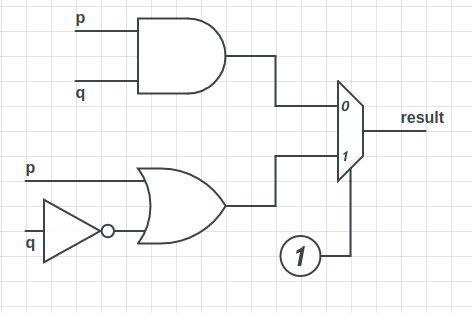
\includegraphics[scale=0.5]{circuit.png}
	\caption{Combinational Circuit}
	\label{fig: circuit}
	
\end{figure*}

In Figure \ref{fig: circuit}, the two statements are used as input. The circuit has 3 gates as AND, OR and NOT operators. It has also a 2x1 multiplexer\footnote{https://www.geeksforgeeks.org/multiplexers-in-digital-logic/} which provides to select one of the two options. 
\subproblem{a} Write the sentence that "result" output has.
\solution
\newline
\newline
result = $(p\wedge q).\neg s + (p\vee \neg q).s$
\newline
If s = 0 the result is that "It is sunny and the flowers are blooming."
\newline
If s = 1 the result is that "It is sunny or the flowers are not blooming."
\newline
then the result is that s=1, so "It is sunny or the flowers are not blooming."
\newline
\subproblem{b} Convert Figure \ref{fig: circuit} to an algorithm which you can write in any programming language that you prefer (including pseudocode).
\solution
\newline
\newline
$include <iostream>$ // including library for function cout
\newline
using namespace std;
\newline
int main(){
\newline
//putting the sentence "it is sunny" into the string p\newline
//putting the sentence "the flowers are blooming." into the string q\newline
string p="It is sunny", q="The flowers are blooming.";\newline\newline
// putting the result from 'and' gate into the firstGate string\newline
//$p\wedge q$
\newline
string firstGate = "It is sunny and the flowers are blooming.";
\newline
// putting the result from 'or' gate into the firstGate string
\newline
//$p\vee \neg q$
\newline
string secondGate = "It is sunny or the flowers are not blooming.";
\newline

//according to result = $(p\wedge q).\neg s + (p\vee \neg q).s$ formula
\newline
// if s is zero, then first statement is executed.
\newline
    if(s == 0)
\newline\newline
        cout $<<$ firstGate
\\newline
//according to result = $(p\wedge q).\neg s + (p\vee \neg q).s$ formula
\newline
//if s is one, then first statement is executed.
\newline
    else
\newline
        cout $<<$ secondGate;
\newline
return 0;
}\newline

\end{document}